\documentclass[11pt,a4paper]{article}

\usepackage{fontspec}
\usepackage[margin=2.0cm]{geometry}
\usepackage{amsmath}
\usepackage{booktabs}
\usepackage{tabularx}
\usepackage{enumitem}
\usepackage{fancyvrb}
\usepackage{xcolor}
\usepackage{tikz}
\usepackage{graphicx}
\usepackage[hidelinks]{hyperref}

\setlist{itemsep=1pt,topsep=3pt}
\setlength{\parindent}{0pt}
\setlength{\parskip}{5pt}
\fvset{fontsize=\small}

% ---------------------------------------------------------------------------
% TA: fill in after calibration (minimum whitespace ratio of the hidden cases,
% in percent).
\newcommand{\WSMIN}{5}
% ---------------------------------------------------------------------------
\newcommand{\WSMINbox}{\WSMIN}
\newcommand{\kw}[1]{\texttt{#1}}
\newcommand{\TBD}{\colorbox{yellow}{\textbf{TBD}}}

\title{\textbf{Lab3 -- Fixed-Outline Floorplanning\\with Soft Blocks and Placement Constraints}}
\author{Physical Design Automation, Fall 2026}
\date{Release: 2026/11/10 \qquad Deadline: 2026/11/23 23:59}

\begin{document}
\maketitle

% ===========================================================================
\section{Introduction}

Floorplanning decides the shape and the location of every block of a chip
inside a given outline. In a modern SoC many blocks have a flexible shape with
only an area budget, some have a fixed shape, some are already placed, and
designers attach placement constraints such as ``these blocks must have the
same shape'' or ``this block must touch the left edge''. This lab is a
simplified variant of Problem~C of the ICCAD 2026 CAD Contest (\emph{The
FloorSet Challenge: Data-Driven SoC Floorplanning}, Intel):
\begin{itemize}
  \item the outline is fixed and given in the input;
  \item blocks are soft, fixed-shape, or preplaced rectangles, and no block
        may be rotated;
  \item the placement constraints are MIB groups and boundary constraints;
  \item every coordinate and dimension is an integer.
\end{itemize}
Implement a C++ floorplanner that places every block inside the outline without
overlap, minimizes the wirelength, and satisfies as many MIB groups and boundary
constraints as possible. Any method is allowed. There is no ranking between
students: each test case is scored by the verifier against fixed thresholds
(Section~\ref{sec:scoring}).

% ===========================================================================
\section{Problem Definition}

\paragraph{Outline and blocks.} The outline is a $W \times H$ rectangle with
its lower-left corner at $(0,0)$. A block is a rectangle with lower-left corner
$(x,y)$, width $w$, and height $h$; it occupies $[x,x+w]\times[y,y+h]$, and
$x,y,w,h$ are integers. Each block is one of:
\begin{itemize}
  \item \textbf{Soft block:} only an area target $a$ is given. You choose
        integer $w,h$ subject to the area tolerance $100\cdot|wh-a|\le a$ and
        the aspect ratio bound $Rh\ge w$ and $Rw\ge h$ (that is,
        $1/R\le h/w\le R$; $R=3$ in all released cases).
  \item \textbf{Fixed-shape block:} $w,h$ are given; you choose the position.
  \item \textbf{Preplaced block:} $w,h,x,y$ are all given.
\end{itemize}
A placement is \emph{feasible} when every block lies inside the outline
($x\ge0$, $y\ge0$, $x+w\le W$, $y+h\le H$) and no two blocks overlap; blocks
$i,j$ overlap when $\max(x_i,x_j)<\min(x_i+w_i,x_j+w_j)$ and
$\max(y_i,y_j)<\min(y_i+h_i,y_j+h_j)$. Touching is allowed. The
\emph{whitespace ratio} of a case is
$1-\bigl(\sum_{\text{soft}} a_b+\sum_{\text{fixed, preplaced}} w_b h_b\bigr)/(WH)$.

\paragraph{Wirelength.} A terminal is a fixed point on the outline border. A
connection joins two endpoints (block--block or block--terminal) with an
integer weight $c$. The position of a block is its centroid
$(x+w/2,\;y+h/2)$; the position of a terminal is its own point. The wirelength
is the weighted sum of Manhattan distances over all connections,
\[
  \mathrm{WL}=\sum_{\text{connections }(a,b,c)}
  c\cdot\bigl(|c_x(a)-c_x(b)|+|c_y(a)-c_y(b)|\bigr),
\]
which is always a multiple of $0.5$. The verifier computes it exactly.

\paragraph{Placement constraints.} An \emph{MIB group} is a set of soft blocks
with identical area targets; it is satisfied when all members have identical
$(w,h)$ (their positions are independent). A \emph{boundary constraint}
requires a block to touch an outline edge:
\begin{center}
\begin{tabular}{llll}
  \toprule
  \kw{LEFT}: $x=0$ & \kw{RIGHT}: $x+w=W$ & \kw{BOTTOM}: $y=0$ & \kw{TOP}: $y+h=H$ \\
  \bottomrule
\end{tabular}
\end{center}
A \emph{corner constraint} lists two adjacent edges and requires both, that is,
the block contains that corner of the outline. These are \emph{scored
constraints}: violating them keeps the output feasible but loses points.

% ===========================================================================
\section{Input Format}

The input is read as whitespace-separated tokens, so line breaks are not
significant. Sections appear in this order, and each count line is followed by
exactly that many records. Text after \kw{//} below is explanation only.

\begin{Verbatim}[frame=single,fontsize=\small]
OUTLINE <W> <H>
WLTHRESHOLD <T>                        // wirelength threshold used for scoring
ASPECTRATIO <R>                        // aspect ratio bound of soft blocks
BLOCKS <n>
SOFT <name> <area>                     // one of these three record types
FIXED <name> <w> <h>                   //   per block, kinds in any order;
PREPLACED <name> <w> <h> <x> <y>       //   n records in total
TERMINALS <r>
TERMINAL <name> <x> <y>                // r records
CONNECTIONS <m>
CONN <name1> <name2> <weight>          // m records
MIBS <q>
MIB <k> <name1> ... <namek>            // q records, k members each
BOUNDARIES <p>
BOUNDARY <name> <EDGE> [<EDGE>]        // p records; EDGE: LEFT RIGHT TOP BOTTOM
\end{Verbatim}

Every input file satisfies the following guarantees.
\begin{itemize}
  \item All numbers are integers except $T$, a positive multiple of $0.5$
        printed with one decimal (for example \kw{123456.5}). $T$ is a
        reference wirelength obtained by the TA's floorplanner on that case.
        $R=3$. Names contain no whitespace, are unique across blocks and
        terminals, and are never an edge keyword.
  \item Bounds: every coordinate and dimension is in $[0,100000]$;
        $n\le200$, $r\le100$, $m\le1000$, $q\le20$, $p\le100$,
        $1\le\mathit{weight}\le10$; $10000\le\mathit{area}\le WH\le10^{10}$.
        Coordinates fit in 32-bit integers, but areas, their products, and the
        wirelength can exceed $2^{31}$: use 64-bit integers.
  \item Preplaced blocks lie strictly inside the outline and do not overlap
        each other. Terminals lie on the outline border.
  \item \kw{CONN}: at least one endpoint is a block; never a block to itself;
        each unordered pair appears at most once.
  \item \kw{MIB}: $k\ge2$; members are soft blocks with identical area
        targets; a block is in at most one group.
        \kw{BOUNDARY}: two edges are always adjacent; only soft and fixed-shape
        blocks; at most one record per block; at most 4 corner constraints per
        case.
  \item Every case has a known feasible solution that satisfies every MIB
        group and every boundary constraint.
\end{itemize}

% ===========================================================================
\section{Output Format}

The output is read line by line: the first non-blank line is
\kw{WIRELENGTH <wl>}, the second is \kw{BLOCKS <n>}, and each of the next $n$
non-blank lines holds one block with exactly five tokens. Blank lines are
ignored; a record split over several lines, or several records on one line,
is rejected.

\begin{Verbatim}[frame=single,fontsize=\small]
WIRELENGTH <wl>
BLOCKS <n>
<name> <x> <y> <w> <h>                 // n lines, in any order
\end{Verbatim}

\kw{<wl>} is the wirelength of your placement as a plain decimal number (for
example \kw{1625.0}); it must match the verifier's value within $0.01$,
otherwise the WL score of the case is 0. \kw{<n>} is the number of blocks in
the input. \kw{<x> <y>} is the lower-left corner and \kw{<w> <h>} the size of
the block; all four are integers. Every input block appears exactly once, and
there are no unknown names.

% ===========================================================================
\section{Example}
\label{sec:example}

A toy case with six blocks (three soft, two fixed-shape, one preplaced), two
terminals, seven connections, one MIB group $\{S1,S2\}$, and two boundary
constraints: \kw{F1 LEFT BOTTOM} (a corner) and \kw{S3 RIGHT}.

\begin{center}
\begin{minipage}[t]{0.46\textwidth}
\textbf{Input}
\VerbatimInput[frame=single,fontsize=\footnotesize]{../cases/toy/toy.in}
\end{minipage}\hfill
\begin{minipage}[t]{0.48\textwidth}
\textbf{Output}
\VerbatimInput[frame=single,fontsize=\footnotesize]{../cases/toy/toy.out}
\vspace{2pt}
\resizebox{\linewidth}{!}{% Generated by tools/plot_tikz.py -- do not edit by hand.
% Needs \usepackage{tikz}; no TikZ libraries required.
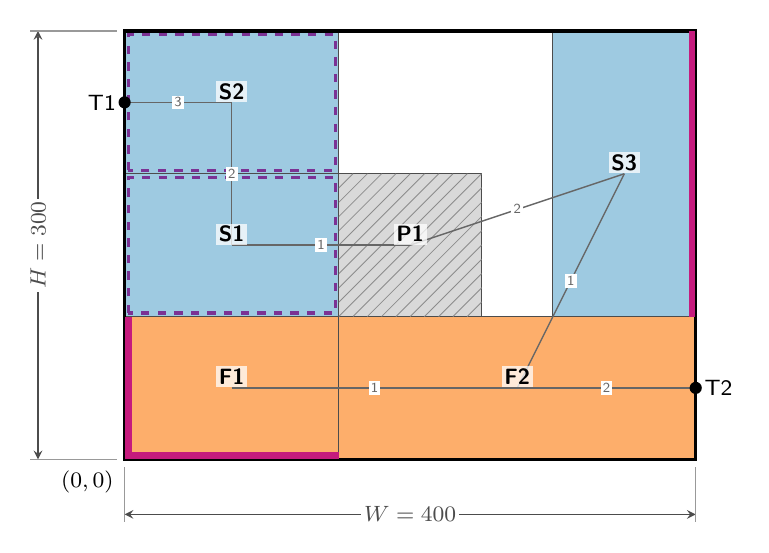
\begin{tikzpicture}[x=0.0015\textwidth,y=0.0015\textwidth,font=\sffamily]
\definecolor{lab3soft}{HTML}{9ECAE1}
\definecolor{lab3fixed}{HTML}{FDAE6B}
\definecolor{lab3preplaced}{HTML}{D9D9D9}
\definecolor{lab3mib0}{HTML}{7B3294}
\definecolor{lab3mib1}{HTML}{008837}
\definecolor{lab3mib2}{HTML}{E66101}
\definecolor{lab3mib3}{HTML}{0571B0}
\definecolor{lab3mib4}{HTML}{CA0020}
\definecolor{lab3mib5}{HTML}{5E3C99}
\definecolor{lab3mib6}{HTML}{1B7837}
\definecolor{lab3mib7}{HTML}{B35806}
\definecolor{lab3mib8}{HTML}{2166AC}
\definecolor{lab3mib9}{HTML}{D6604D}
\definecolor{lab3mib10}{HTML}{542788}
\definecolor{lab3mib11}{HTML}{01665E}
\definecolor{lab3bound}{HTML}{C51B7D}
\fill[white] (0,0) rectangle (400,300);
\filldraw[fill=lab3soft,draw=black!70,line width=0.4pt] (0,100) rectangle (150,200);
\filldraw[fill=lab3soft,draw=black!70,line width=0.4pt] (0,200) rectangle (150,300);
\filldraw[fill=lab3soft,draw=black!70,line width=0.4pt] (300,100) rectangle (400,300);
\filldraw[fill=lab3fixed,draw=black!70,line width=0.4pt] (0,0) rectangle (150,100);
\filldraw[fill=lab3fixed,draw=black!70,line width=0.4pt] (150,0) rectangle (400,100);
\filldraw[fill=lab3preplaced,draw=black!70,line width=0.4pt] (150,100) rectangle (250,200);
\begin{scope}
\clip (150,100) rectangle (250,200);
\draw[black!45,line width=0.3pt] (50,100) -- (150,200);
\draw[black!45,line width=0.3pt] (60,100) -- (160,200);
\draw[black!45,line width=0.3pt] (70,100) -- (170,200);
\draw[black!45,line width=0.3pt] (80,100) -- (180,200);
\draw[black!45,line width=0.3pt] (90,100) -- (190,200);
\draw[black!45,line width=0.3pt] (100,100) -- (200,200);
\draw[black!45,line width=0.3pt] (110,100) -- (210,200);
\draw[black!45,line width=0.3pt] (120,100) -- (220,200);
\draw[black!45,line width=0.3pt] (130,100) -- (230,200);
\draw[black!45,line width=0.3pt] (140,100) -- (240,200);
\draw[black!45,line width=0.3pt] (150,100) -- (250,200);
\draw[black!45,line width=0.3pt] (160,100) -- (260,200);
\draw[black!45,line width=0.3pt] (170,100) -- (270,200);
\draw[black!45,line width=0.3pt] (180,100) -- (280,200);
\draw[black!45,line width=0.3pt] (190,100) -- (290,200);
\draw[black!45,line width=0.3pt] (200,100) -- (300,200);
\draw[black!45,line width=0.3pt] (210,100) -- (310,200);
\draw[black!45,line width=0.3pt] (220,100) -- (320,200);
\draw[black!45,line width=0.3pt] (230,100) -- (330,200);
\draw[black!45,line width=0.3pt] (240,100) -- (340,200);
\end{scope}
\draw[lab3mib0,dashed,line width=1.2pt] (2.5,102.5) rectangle (147.5,197.5);
\draw[lab3mib0,dashed,line width=1.2pt] (2.5,202.5) rectangle (147.5,297.5);
\draw[black!60,line width=0.5pt] (75,150) -- node[fill=white,inner sep=0.8pt,font=\sffamily\tiny] {2} (75,250);
\draw[black!60,line width=0.5pt] (75,150) -- node[fill=white,inner sep=0.8pt,font=\sffamily\tiny] {1} (200,150);
\draw[black!60,line width=0.5pt] (75,250) -- node[fill=white,inner sep=0.8pt,font=\sffamily\tiny] {3} (0,250);
\draw[black!60,line width=0.5pt] (200,150) -- node[fill=white,inner sep=0.8pt,font=\sffamily\tiny] {2} (350,200);
\draw[black!60,line width=0.5pt] (75,50) -- node[fill=white,inner sep=0.8pt,font=\sffamily\tiny] {1} (275,50);
\draw[black!60,line width=0.5pt] (275,50) -- node[fill=white,inner sep=0.8pt,font=\sffamily\tiny] {2} (400,50);
\draw[black!60,line width=0.5pt] (350,200) -- node[fill=white,inner sep=0.8pt,font=\sffamily\tiny] {1} (275,50);
\node[font=\sffamily\footnotesize\bfseries,fill=white,fill opacity=0.75,text opacity=1,inner sep=1pt,above] at (75,150) {S1};
\node[font=\sffamily\footnotesize\bfseries,fill=white,fill opacity=0.75,text opacity=1,inner sep=1pt,above] at (75,250) {S2};
\node[font=\sffamily\footnotesize\bfseries,fill=white,fill opacity=0.75,text opacity=1,inner sep=1pt,above] at (350,200) {S3};
\node[font=\sffamily\footnotesize\bfseries,fill=white,fill opacity=0.75,text opacity=1,inner sep=1pt,above] at (75,50) {F1};
\node[font=\sffamily\footnotesize\bfseries,fill=white,fill opacity=0.75,text opacity=1,inner sep=1pt,above] at (275,50) {F2};
\node[font=\sffamily\footnotesize\bfseries,fill=white,fill opacity=0.75,text opacity=1,inner sep=1pt,above] at (200,150) {P1};
\draw[black,line width=1.2pt] (0,0) rectangle (400,300);
\draw[lab3bound,line width=2.4pt,line cap=butt] ([xshift=1.3pt]0,0) -- ([xshift=1.3pt]0,100);
\draw[lab3bound,line width=2.4pt,line cap=butt] ([yshift=1.3pt]0,0) -- ([yshift=1.3pt]150,0);
\draw[lab3bound,line width=2.4pt,line cap=butt] ([xshift=-1.3pt]400,100) -- ([xshift=-1.3pt]400,300);
\fill[black] (0,250) circle (2.2pt);
\node[anchor=east,font=\sffamily\footnotesize,inner sep=3pt] at (0,250) {T1};
\fill[black] (400,50) circle (2.2pt);
\node[anchor=west,font=\sffamily\footnotesize,inner sep=3pt] at (400,50) {T2};
\draw[black!70,<->,>=stealth] ([yshift=-7mm]0,0) -- node[fill=white,inner sep=1pt,font=\sffamily\footnotesize] {$W=400$} ([yshift=-7mm]400,0);
\draw[black!40] ([yshift=-1mm]0,0) -- ([yshift=-8mm]0,0);
\draw[black!40] ([yshift=-1mm]400,0) -- ([yshift=-8mm]400,0);
\draw[black!70,<->,>=stealth] ([xshift=-11mm]0,0) -- node[fill=white,inner sep=1pt,font=\sffamily\footnotesize,rotate=90] {$H=300$} ([xshift=-11mm]0,300);
\draw[black!40] ([xshift=-1mm]0,0) -- ([xshift=-12mm]0,0);
\draw[black!40] ([xshift=-1mm]0,300) -- ([xshift=-12mm]0,300);
\node[anchor=north east,font=\sffamily\footnotesize,inner sep=1pt] at ([xshift=-1mm,yshift=-1mm]0,0) {$(0,0)$};
\end{tikzpicture}
}
{\footnotesize Blue: soft blocks; orange: fixed-shape blocks; grey hatched:
preplaced block. Dashed purple: the MIB group $\{S1,S2\}$; thick magenta bars:
required edges of the boundary constraints. Dots: terminals; lines:
connections between centroids, labeled with their weights.\par}
\end{minipage}
\end{center}

S1 and S2 are both $150\times100$ (area $15000$, ratio $2/3$), S3 is
$100\times200$; F1 touches $x=0$ and $y=0$, S3 touches $x+w=400=W$. The
centroids are S1 $(75,150)$, S2 $(75,250)$, S3 $(350,200)$, F1 $(75,50)$,
F2 $(275,50)$, P1 $(200,150)$, and the terminals are T1 $(0,250)$,
T2 $(400,50)$. For example, \kw{CONN P1 S3 2} contributes
$2\cdot(|200-350|+|150-200|)=400$ and the block--terminal connection
\kw{CONN S2 T1 3} contributes $3\cdot(|75-0|+|250-250|)=225$; the seven
connections sum to $1625$. (Had S2 been $151\times99$ at the same corner, its
centroid would be $(75.5,249.5)$: this is how half-integer wirelengths arise.)
The verifier report for this output is:
\begin{Verbatim}[frame=single,fontsize=\footnotesize]
$ ./verifier toy.in toy.out
Gate checks:
  1. Output format          PASS
  2. Block names            PASS
  3. Positive size          PASS
  4. Fixed/preplaced shape  PASS
  5. Soft area tolerance    PASS
  6. Soft aspect ratio      PASS
  7. Inside outline         PASS
  8. Overlap-free           PASS
Result: FEASIBLE
Reported WL   1625.0
Computed WL   1625.0
Threshold T   1700.0
Gate          10.00 / 10
WL score      5.00 / 5
Boundary      3.00 / 3  (2/2 satisfied)
MIB           2.00 / 2  (1/1 satisfied)
Total 20.00 / 20
\end{Verbatim}
A feasible output that violates a scored constraint keeps the gate points and
loses only that item: for instance, with S2 reshaped to $151\times99$ (and
\kw{WIRELENGTH 1628.0}) the MIB group is no longer satisfied and the case
scores $18.00/20$.

% ===========================================================================
\section{Scoring and Test Cases}
\label{sec:scoring}

There are 5 cases, 1 public (released with the assignment) and 4 hidden, each
worth 20 points as in Table~\ref{tab:scoring}, for a total of 100 points. WL,
boundary, and MIB are scored only on a feasible output. If $p=0$ or $q=0$,
that item gives full points (released cases have $p,q>0$).

\begin{table}[htbp]
\centering
\caption{Scoring of one case (20 points).}
\label{tab:scoring}
\renewcommand{\arraystretch}{1.15}
\begin{tabularx}{\textwidth}{@{}l c X@{}}
  \toprule
  Item & Points & Rule \\
  \midrule
  Gate & 10 &
    All of the following must hold; \textbf{any failure scores 0 for the whole
    case}.
    \begin{enumerate}[nosep,leftmargin=1.4em,label=\arabic*.]
      \item The output parses (header lines, $n$ block lines of five tokens,
            integers where required).
      \item Every input block appears exactly once; no unknown names.
      \item $w>0$ and $h>0$ for every block.
      \item Fixed-shape blocks have their given $(w,h)$; preplaced blocks
            their given $(x,y,w,h)$.
      \item Soft area tolerance $100\cdot|wh-a|\le a$.
      \item Soft aspect ratio $Rh\ge w$ and $Rw\ge h$.
      \item Inside the outline.
      \item Overlap-free (touching allowed).
      \item Runtime at most 120\,s and single-threaded execution.
    \end{enumerate}
    The verifier checks 1--8 and prints \kw{FEASIBLE} exactly when they hold;
    check~9 is applied by the TA's grading script. \\
  \midrule
  WL & 5 &
    $0$ if the reported \kw{<wl>} differs from the computed WL by more than
    $0.01$; otherwise, with $T$ the \kw{WLTHRESHOLD} of the case,
    \[
      S_{\mathrm{WL}} =
      \begin{cases}
        5 & \mathrm{WL} \le T,\\[2pt]
        5 \cdot \dfrac{1.05\,T - \mathrm{WL}}{0.05\,T} & T < \mathrm{WL} \le 1.05\,T,\\[8pt]
        0 & \mathrm{WL} > 1.05\,T.
      \end{cases}
    \] \\
  \midrule
  Boundary & 3 &
    $3\cdot\mathit{satisfied}/p$; a block is satisfied only when it touches
    all of its listed edges. \\
  \midrule
  MIB & 2 &
    $2\cdot\mathit{satisfied}/q$; a group is satisfied when all members have
    identical $(w,h)$. \\
  \bottomrule
\end{tabularx}
\end{table}

The verifier prints each gate check as PASS or FAIL with the first violation
(for example \kw{Overlap: S3 P1}), then the reported WL, the computed WL, $T$,
and the item scores. It exits with status 0 on a feasible output and 1
otherwise. The grading verifier is the same binary as the released one.

\paragraph{Hidden cases.} The hidden cases follow the same format and
guarantees as the public case: at most 200 blocks; every constraint type
(soft, fixed-shape, and preplaced blocks, terminals, MIB groups, and boundary
constraints including corners) appears in every case; whitespace ratio
approximately \WSMINbox\,\% or more; difficulty increases with the number of blocks, tighter
whitespace, and higher constraint density. Do not tune your program to the
public case only.

% ===========================================================================
\section{Execution}

Provide a \kw{Makefile} that builds an executable named \kw{Lab3}. The TA
compiles and runs your program, then checks the output with the released
verifier (use \kw{chmod +x verifier} the first time if needed):
\begin{Verbatim}[frame=single]
make
./Lab3 <input_file> <output_file>
./verifier <input_file> <output_file>
\end{Verbatim}
\begin{itemize}
  \item Runtime limit: \textbf{120 seconds wall-clock per case}, measured on
        the course workstation (CPU: Intel Xeon E5-2630 v4 @ 2.20\,GHz,
        OS: Rocky Linux 8.10, g++: 11.2.0). Exceeding
        it fails the gate.
  \item The program must be \textbf{single-threaded}: no \kw{std::thread},
        OpenMP, \kw{fork}, or any other parallel work. A violation fails the
        gate.
  \item Compile and test your final version on the course workstation. A
        submission that fails to compile or run there receives 0 points.
\end{itemize}

% ===========================================================================
\section{Submission}

\begin{enumerate}
  \item Put all required files in a folder named with your student ID:
\begin{Verbatim}
Student_ID/
    source code (.cpp, .h)
    Makefile
    readme.txt          (how to build and run your program)
\end{Verbatim}
  \item Archive the folder in a Linux environment; the archive name must be
        your student ID. For example, student 310510161 submits
        \kw{310510161/} containing \kw{Lab3.cpp}, \kw{Makefile}, and
        \kw{readme.txt}, archived with
\begin{Verbatim}
tar cvf 310510161.tar 310510161
\end{Verbatim}
  \item Upload \kw{Student\_ID.tar} to e3. A submission in any other format
        receives 0 points. No written report is required.
\end{enumerate}

\begin{itemize}
  \item Deadline: \textbf{2026/11/23 23:59}. Late submissions lose 20\% of
        the score per day, and any part of a day counts as a full day: a
        submission by 2026/11/24 23:59 loses 20\%, by 2026/11/25 23:59 loses
        40\%, and so on.
  \item You may use AI tools, but you must write and submit your own code.
        All submissions are checked for similarity; if two are highly similar,
        both receive 0 points after confirmation.
\end{itemize}

\end{document}
